\chapter{Cryptographic techniques for cybersecurity}


\section{Cryptography}

\begin{figure}[h]
    \centering
    \includegraphics[page = 2,trim = 0.5cm 3cm 1cm 5cm, clip, width = 0.55\textwidth]{\slides}
\end{figure}


The most used technique to achieve protection for many centuries is \textbf{cryptography}; a mathematical technique that involves algorithms for encryption and decryption:
\begin{itemize}
    \item the encryption algorithm takes a message (in clear) and transforms it in such a way that it becomes unintelligible;
    \item to recover the original text, the decryption algorithms make it readable again.
\end{itemize}
Next to the algorithms, \textbf{key-1} is needed for encryption and \textbf{key-2} for decryption, both of which are streams of bits.
Cryptography is used in communication and for data storage (for example, to store data on disks without permission to read them except for authorized users). The common terminology used in cryptography includes two other keywords:
\begin{itemize}
    \item \textbf{Plaintext} or \textbf{cleartext}: the unencrypted message, typically referred to as \textbf{P};
    \item \textbf{Ciphertext}: the encrypted message, typically referred to as \textbf{C}. Note that in some countries, the term "encrypted" may sound offensive for religious reasons (related to the cult of the dead); in such cases, "\emph{enciphered}" is preferred.
\end{itemize}


\subsection{Cryptography's strength (Kerchoffs' principle)}
Kerckhoffs' Principle (1883) states that \ul{the security of a cryptosystem must lie in the choice of its keys only};
everything else (including the algorithm itself) should be considered of public knowledge.
However, this principle relies on the fact that the keys have the following properties.
\begin{itemize}
    \item Are kept \textbf{secret};
    \item Are managed only by \textbf{trusted systems};
    \item Are of \textbf{adequate length} % TODO: cross-reference this
\end{itemize}

If these properties are met,
not only it has no importance that the encryption and decryption algorithms are kept secret, but it is better to
make the algorithms public so that they can be widely analysed, and their possible flaws and vulnerabilities identified.

\subsection*{Security through obscurity (STO)}
The Kerckhoffs' Principle is related to the concept of \textbf{Security through obscurity}: it means that a system is protected, but the details on how it has been protected are not disclosed.\\
Generally, \ul{this alone is not considered a valid security mechanism} because if someone discovers how the system has been protected (and we have seen that there are also non-technical ways by which this can be achieved), it is no longer secure.

For this reason, we say that \emph{"Security through obscurity is as bad with computer systems as it is with women"}.
\begin{quote}
    "Men try to hide things from women, but when they discover the truth, it is worse than if they had known it from the beginning"
\end{quote}
\begin{flushright}
    (Antonio Lioy)
\end{flushright}
\emph{Editor's note:} don't hide things from your partner, regardless of gender.


However, there is a category of people (such as military men) which tend to apply STO, but as an \ul{additional
    layer}. It is possible to use STO as a layer only if a really strong algorithm is used (but not a secret one).



\section{Symmetric cryptography}
Depending on which relation exists between key-1 and key-2 there are different kinds of cryptography.

\subsection*{Secret key / symmetric cryptography}
\begin{figure}[h]
    \centering
    \includegraphics[page = 6,trim = 2.5cm 3cm 2.5cm 13cm, clip, width = 0.55\textwidth]{\slides}
    \caption{Symmetric cryptography}
    \label{fig:cap2slide6}
\end{figure}

It is so named because \textbf{only a single key} is shared by the sender and receiver. In the diagram, there is a plaintext used as input for the encryption (E) block, along with the key. The result is a comprehensible text that is transmitted to the receiver. To retrieve the original text, the decryption (D) block algorithm is used with the same key that was used for encrypting the initial text. If a different key is used, an output is generated, but it will be incorrect (and typically understandable).

The formulas used are as follows.

% TODO: fix these formulas 
\begin{align*}
    K_1 & = K_2 = K                                    \\
    C   & = enc(K,P) \quad \text{or} \quad C = \{P\} K \\
    P   & = dec(K,C) = enc^{-1} (K,C)
\end{align*}
Note that $C = \{P\} K$ means "encrypt the plaintext P using the key K".


% TODO: cross reference "Key distribution for symmetric cryptography"
The issue in the diagram (Figure \ref{fig:cap2slide6}) is represented by the dashed line: how can the key be securely shared between the sender and receiver?
We'll see it in \textit{Key distribution for symmetric cryptography}.


\subsection{Block algorithms}
\begin{figure}[h]
    \centering
    \includegraphics[page = 7,trim = 1cm 1.5cm 1cm 4cm, clip, width = 0.55\textwidth]{\slides}
    \caption{Some famous symmetric encryption algorithms (block)}
\end{figure}

There are many algorithms, and the table on the left represents just a small selection. \\
The first column provides the name, the second indicates the key length, and the third specifies the basic unit each algorithm can encrypt. These algorithms are referred to as "\textbf{block algorithms}" because they operate on a fixed number of bits.

The \textbf{DES} algorithm, once a standard for many years, is now considered obsolete and should never be used.

The most commonly used algorithm of this kind is \textbf{AES}, currently recognized as the state of the art (the strongest).

\textbf{RC5} performs optimally when the block size is double the word size of the CPU architecture (e.g., 64-bit architecture -> 128-bit block) on which the algorithm is implemented.

Why are there so many algorithms? Because there are various types of computers, and many algorithms are not suitable for low CPU power.


\paragraph*{The EX-OR (XOR) function}
\begin{wrapfigure}{r}{0.255\textwidth}
    \centering
    \includegraphics[page = 8,trim = 21cm 7.2cm 0.5cm 8.5cm, clip, width = 0.25\textwidth]{\slides}
    \caption{XOR function}
\end{wrapfigure}

It is the ideal "confusion" operator, available on all CPU. \\
The peculiarity of this truth table is that it has 50\% of
0 and 50\% of 1:
if XOR is performed with 2 random inputs (probability 0:1 = 50\% : 50\%),
then the output will also be equally random; while, for example, AND is more likely to produce 0.
That means that XOR does not change the probability distribution of the input, even though it generates different outputs.
Some properties:
\begin{itemize}
    \item if $A \oplus B = Z$ \\
          then $Z \oplus B = A$  or $Z \oplus A = B$
    \item $A \oplus 0 = A$ \\
          $A \oplus 1 = \overline{A}$\\
          $A \oplus A = 0$\\
          $A \oplus \overline{A} = 1$
\end{itemize}


\subsubsection{DES}
\textbf{DES} stands for "\textbf{Data Encryption Standard}" and it is a standard defined by \textit{FIPS 46/2} (Federal Information Processing Standard, the body responsible for setting standards for the American government). The modes for applying DES to data that is not equally divided into blocks are mentioned in the FIPS 81 standard.

DES is a unique algorithm because it has a 64-bit key, but its effective strength is equivalent to that of a \textbf{56-bit key}, as 8 bits are used for parity. This means that when a key is generated for the DES algorithm, only 56 bits are truly random, and every 7 bits, the algorithm inserts a bit that serves as the parity of the preceding 7 bits. When an attacker attempts to crack DES, they only need to discover these 56 truly random bits. DES is the only algorithm that distinguishes between actual (bits used to create the key) and effective (total number of bits) bits.

Developed in the 1960s, DES uses a \textbf{64-bit data block}, a size chosen when computers were less powerful. To perform all the necessary mathematical computations, a special-purpose unit called an \textbf{encryption processor} was created because DES relies on it to perform:

\begin{itemize}
    \item \textbf{XOR}: which is not a problem → elementary operation;
    \item \textbf{Shift}: not a problem → elementary operation;
    \item \textbf{Permutation}: expensive operation. The permutation is not random, there are several ones, but still implementing that was much more efficient if done directly in hardware.
\end{itemize}

\subsubsection{Triple DES (3DES, TDES)}
Triple DES is the repeated application of DES (three times). It is possible to use two or three different 56bit keys.
Typically, the process involves taking the input, encrypting it, and then repeating this operation two more times, using the output of the previous encryption as the input for the next encryption (resulting in three consecutive encryptions).

Normally, it is implemented in \textbf{EDE} mode, which, in its standard form, requires \ul{two keys}: the plaintext is first encrypted with key-1, then the decryption algorithm is applied to the output using key-2 (which does not actually decrypt but applies another transformation), and finally, this last output is encrypted again using key-1.
This mode was chosen because setting $K_1 = K_2 = K_3$ allows for the implementation of the simple DES in EDE mode.
Thus, both EEE and EDE work equally well. It has been shown that 3DES with two keys can have lower security guarantees than expected.

In particular, denoting $K_{eq}$ as the equivalent key obtained by applying the discussed transformations:
\begin{itemize}
    \item \textbf{3DES with 2 keys},
          \(K_{\text{eq}} = 56\) bits if $2^{59}B$ of memory is available, otherwise \(K_{\text{eq}} = 112\) bits:
          \[C' = \text{enc}(K_1, P) \quad C'' = \text{dec}(K_2, C') \quad C = \text{enc}(K_1, C'')\]
    \item \textbf{3DES with 3 keys}, \(K_{\text{eq}} = 112\) bits:
          \[C' = \text{enc}(K_1, P) \quad C'' = \text{dec}(K_2, C') \quad C = \text{enc}(K_3, C'')\]
\end{itemize}

The 3DES is a standard FIPS 46/3 and ANSI X9.52 (family X9 is standard for security in banking and financial
applications).

\begin{figure}[h]
    \centering
    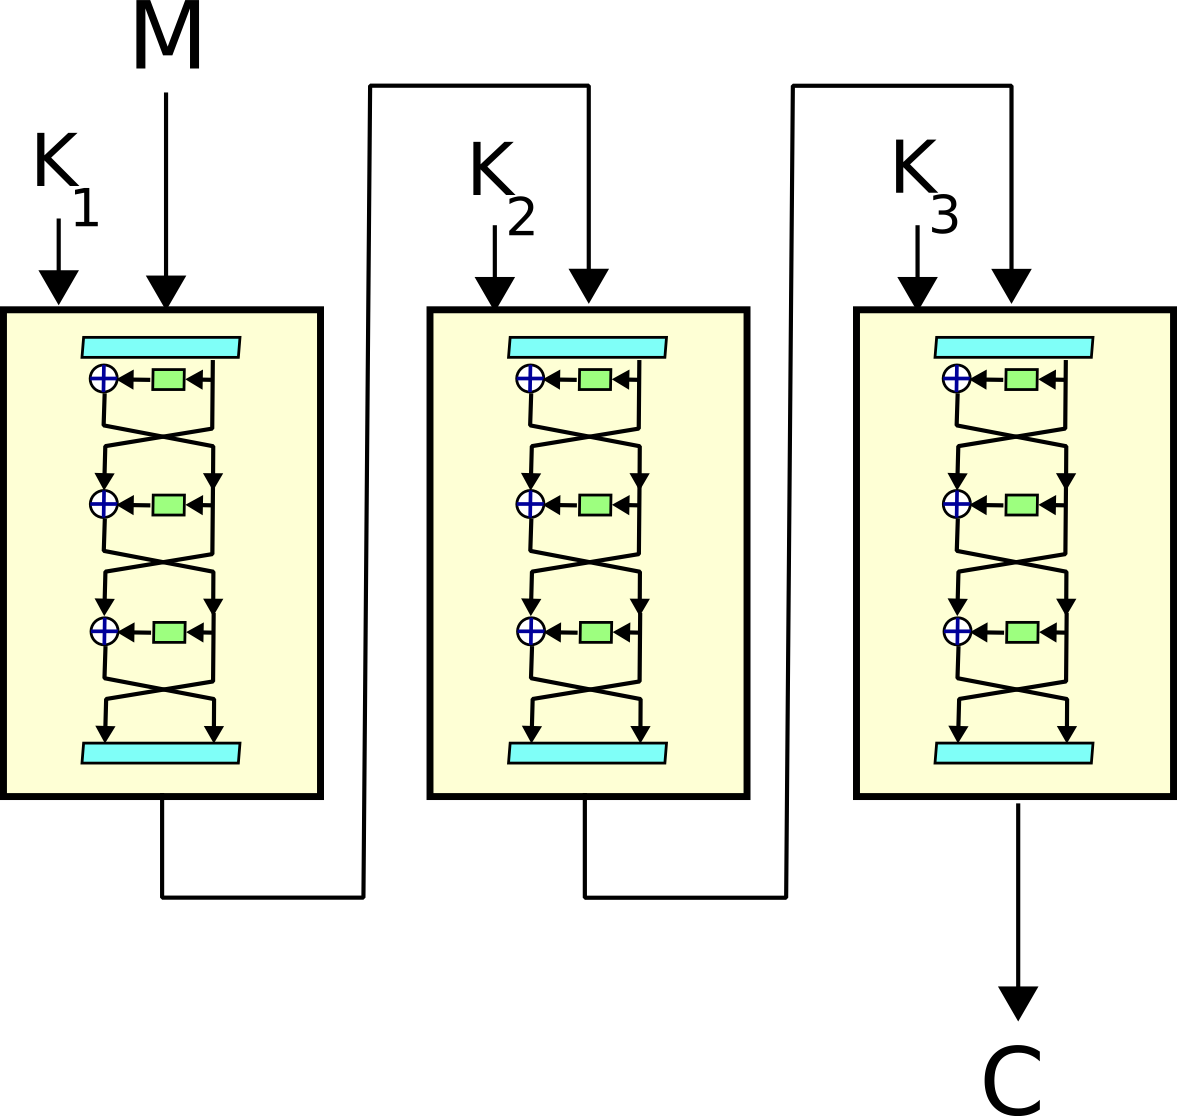
\includegraphics[width = 0.30\textwidth]{chapter2/3des.png}
\end{figure}

\paragraph*{Why not Double DES?}
The double application of any encryption algorithm is susceptible to a \textbf{known-plaintext} attack known as \textit{meet-in-the-middle} see below), which allows for the decryption of data with at most \(2^{N+1}\) attempts (if the keys are \(N\) bits long), instead of the $2^{2n}$ steps one would expect from an ideally secure algorithm with $2n$ bits of key.
If the attacker knows one plaintext, they can execute the attack. For this reason, \textbf{the double version of encryption algorithms is never used} because the computation time doubles, but the effective key length increases by just one bit.

Furthermore, it has been proven that if the base symmetric algorithm is a \href{https://en.wikipedia.org/wiki/Group_(mathematics)}{\underline{group}} , then there exists an equivalent key \(K_3\) such that:

\[
    \text{enc}(K_2, \text{enc}(K_1, P)) = \text{enc}(K_3, P)
\]

This implies that in this case, the time needed for normal encryption/decryption doubles, but not a single bit is gained in terms of \(K_{eq}\).

%TODO: migliora disposizione equazioni
\subparagraph*{Meet-in-the-middle attack}\label{meetinthemiddle}
By hypothesis, N-bit keys are used, and we have known plaintext (\(P\)) and ciphertext (\(C\)) such that
\[C = \text{enc}(K_2, \text{enc}(K_1, P))\] \\
Note that \(\exists M\) such that
\begin{align*}
    M & = \text{enc}(K_1, P) \\
    C & = \text{enc}(K_2, M)
\end{align*}
The attacker computes \(2^N\) values \(X_i = \text{enc}(K_i, P)\) and then computes \(2^N\) values \(Y_j = \text{dec}(K_j, C)\).
The search then involves finding those values \(K_i\) and \(K_j\) such that \(X_i = Y_j\).
There can be "false positives" but these can be easily discarded if more than one \((P, C)\) pair is available.

\begin{figure}[h]
    \centering
    \includegraphics[page = 12,trim = 3cm 3cm 2cm 3cm, clip, width = 0.50\textwidth]{\slides}
\end{figure}

Let's consider a company protecting its communication between Turin and Milan using double DES. If the attacker sniffs the network (and reads the encrypted data), they can send a message over that line (meaning they control the plaintext), and then observe the ciphertext (of the sent plaintext) automatically generated by the security system.
This is a way to obtain a pair of \((P, C)\) without knowing the keys.




\newpage
\subsection{Application of block algorithm}

\textit{How is a block algorithm applied to a data quantity different from the algorithm's block size?}
There are two cases\footnote{The distinction should be: is the \texttt{data size} \textbf{multiple} of the \textit{algorithm's block size}?}:
\begin{enumerate}
    \item \texttt{Data size to encrypt} $>$ \texttt{algorithm's block size}
          \begin{itemize}
              \item \textbf{ECB (Electronic Code Book):} Nowadays considered not secure and must never be used.
              \item \textbf{CBC (Cipher Block Chaining):} Currently the best way to apply an encryption algorithm to data that is bigger than the size of the algorithm's block size.
          \end{itemize}

    \item \texttt{Data size to encrypt} $<$ \texttt{algorithm's block size}
          \begin{itemize}
              \item \textbf{Padding:} Used only when the data size is not exactly a multiple of one block size (e.g., when data is 2.6 blocks long). Note that this technique is not used to pad data that is just shorter than one block size.
                    \begin{itemize}
                        \item \textbf{CTS (CipherText Stealing):} Permits the use of block algorithms without padding, avoiding an increase in the size of the ciphertext compared to the plaintext.
                    \end{itemize}
              \item \textbf{CFB (Cipher FeedBack), OFB (Output Feedback), CTR (Counter mode):} These are application modes for an algorithm, not algorithms themselves.
          \end{itemize}
\end{enumerate}
\textbf{ATTENTION!} These are NOT algorithms; they are application modes for an algorithm.

It is necessary to specify:
the algorithm, the size of key, and if it is a block algorithm, also the mode of the application (e.g., AES-128-CBC).


\subsubsection{ECB}
\paragraph*{Encryption}
This mode splits the plaintext into blocks, and each block is encrypted separately with the key;
that means that, for each block \(i = 0, \ldots, N\),
\[
    C_i = \text{enc}(K, P_i)
\]
\begin{figure}[h]
    \centering
    \includegraphics[page = 14,trim = 8cm 2cm 8cm 12cm, clip, width = 0.30\textwidth]{\slides}
    \caption{Encryption with ECB}
\end{figure}

\underline{It must \textbf{NOT} be used!} [\textit{Lioy said that the exam will not be passed if ECB is used somehow}].
In particular, it must not be used on long messages (any message longer than 1 block) because:
\begin{itemize}
    \item If the attacker is intercepting the ciphertext and exchanges the position of 2 blocks, it is not detected (\textbf{block swapping}). This permits to exchange data inside an encrypted message;
    \item Identical blocks generate identical ciphertexts, hence it is vulnerable to \textbf{known-plaintext attacks}. Plaintext attacks require the precomputation of all possible encryptions of a known plaintext: comparing the encrypted block with all the precomputed possible encryptions, it is possible to figure out what the key is.
\end{itemize}

\subparagraph*{Known-plaintext attack example}
Let us suppose that we want to intercept a message sent by the rector of the Politecnico di Torino. It is possible
to assume that his messages will contain the word “Torino”, so we start encrypting this word with all possible
keys. Next, we can go sniffing the blocks sent by the rector: if any of these blocks is equal to the encryption
of “Torino”, then we can use the key used to obtain that encryption of “Torino” to decrypt the rest of the
message. Some arguments against this method could be: in which way is “Torino” written (e.g., “TORINO”,
“Torino”)? What if “Torino”, since it is shorter than one machine word, is split into different blocks (e.g., \(P_i\) =
“…To”, \(P_{i+1}\) = “rino…”)? The known-plaintext attack is made possible by the fact that usually people exchange
data in a structured format, so that there are metadata that are usually known (e.g., fixed header).


If a Word file is created with just a word, it is big KBs of memory (and not just bytes). This happens because
Word applies a header on the document which is always the same (and always at the beginning of a file). If
the first block of a Word file is encrypted, it can serve as a dictionary for Word files. This means that we do not
even have to guess some plaintext, but just the file format.


\paragraph*{Decryption}
Decryption is a straightforward process as it involves taking the ciphertext block and decrypting it with the corresponding key. In the case of an error in transmission, it only affects the decryption of that specific block, and \textbf{there is no propagation of the error to other blocks}.
\begin{itemize}
    \item For each block, $P_i = \text{enc}^{-1}(K, C_i)$
\end{itemize}
\begin{figure}[h]
    \centering
    \includegraphics[page = 15,trim = 8cm 2cm 8cm 10.5cm, clip, width = 0.30\textwidth]{\slides}
    \caption{Decryption with ECB}
\end{figure}


\subsubsection{CBC (Cipher Block Chaining)}

\paragraph*{Encryption}
This mode resolves all of ECB's problems.
It divides the plaintext into blocks, but before each block is encrypted, it is \textbf{XORed with the ciphertext of the previous block}.
This introduces unpredictability in the encryption process.
However, there is an issue with the first block (which serves as the header of the mentioned file); to apply CBC, an additional element called the \textbf{Initialization Vector (IV)} must be introduced, considered as \(C_0\), with the sole purpose of altering the first plaintext block.

CBC also provides protection against block swapping because if blocks are swapped, the output will be different due to being altered with the incorrect XOR element.
\begin{itemize}
    \item For each block, $C_i = \text{enc}(K, P_i \oplus C_{i-1})$
    \item Requires \textbf{IV}
\end{itemize}


\begin{figure}[H]
    \centering
    \includegraphics[page = 16,trim = 4cm 2cm 4cm 8.5cm, clip, width = 0.55\textwidth]{\slides}
    \caption{CBC encryption}
\end{figure}


\paragraph*{Decryption}
The IV vector needs to be known at the receiver as well because, when the ciphertext is received, the IV must be known to decrypt the first block (since XOR is the inverse operator of itself).
The IV must also be different every time (hopefully random) to avoid being guessed, as its purpose is to make it impossible to precompute the possible encryptions of the first block.
It must also be a \textbf{NONCE} (Number used once), meaning that the IV should be generated and never reused in the future.

In some cases, the IV is sent in clear because even if the attacker knows it, they could start the computation only at that moment, and this is a time-consuming task. Moreover, it will permit the attacker to attack only the sent message, as the next one will have another IV.
The IV can also be sent encrypted using ECB since it is just a block.

Opposed to ECB, \textbf{one error in transmission} generates an error at the
decryption of \textbf{two blocks}. For example, if there's an error in C1, it affects the decryption, causing incorrect P1 and P2. However, P3 remains unaffected because C2 and C3 are needed for its decryption, and they are error-free in this case.


\begin{itemize}
    \item $P_i = \text{enc}^{-1}(K, C_i ) \oplus C_{i-1}$
    \item Requires \textbf{IV} to be known by the receiver
\end{itemize}


\begin{figure}[H]
    \centering
    \includegraphics[page = 17,trim = 4cm 1.5cm 4cm 9.5cm, clip, width = 0.55\textwidth]{\slides}
    \caption{CBC decryption}
\end{figure}



\subsubsection*{Padding (aligning, filling)}
\begin{figure}[H]
    \centering
    \includegraphics[page = 18,trim = 3.5cm 7cm 3.5cm 9cm, clip, width = 0.55\textwidth]{\slides}
\end{figure}
It is not always possible to have the plaintext split into blocks that are all the same size. In the picture, the data consists of two complete blocks and a partial block at the end. To encrypt this small part, a technique called padding is used. Bits are added at the end of the original data until it reaches a multiple of a block.
However, it has some problems since:
\begin{itemize}
    \item The ciphertext gets longer than the plaintext: adding useless data means transmitting / storing more data
          than needed;
    \item Which should be the value of padding bits? How can we distinguish the padding from the original
          plaintext at the receiver?
          The are numerous \textbf{padding techniques}:
          \begin{itemize}
              \item If the length is known or it can be obtained as in the case of a C string, it is possible to add null bytes
                    at the end: \texttt{0x00 0x00 0x00};
              \item The original DES specified to add one "1" bit followed by as many "0" as needed: \texttt{1000000};
              \item One byte with value 128 followed by null bytes: \texttt{0x80 0x00 0x00};
              \item Last byte's value equal to the length of padding: \texttt{0x?? 0x?? 0x03} (3 bytes of padding. The last one
                    has value 3, and the previous has a value to be specified).
                    There are numerous padding techniques available, and the choice of a specific padding method plays a crucial role in preventing or mitigating various types of attacks.
                    Consider the value of other bits (\texttt{0x??})\footnote{do not remember all the techniques, just remember there
                        are many and the proper one must be selected}:
                    \begin{itemize}
                        \item (Schneier) null bytes, e.g., \texttt{0x00 0x00 0x03}
                        \item (SSL/TLS) bytes with value $L$, e.g., \texttt{0x03 0x03 0x03}
                        \item (SSH2) random bytes, e.g., \texttt{0x05 0xF2 0x03}
                        \item (IPsec/ESP) progressive number, e.g., \texttt{0x01 0x02 0x03}
                        \item Byte with value $L-1$, e.g., \texttt{0x02 0x02 0x02}
                    \end{itemize}
          \end{itemize}
\end{itemize}



% TODO L?
\paragraph*{Some notes}
\begin{itemize}
    \item $B$ stands for the size of the algorithm's block
    \item $D$ stands for the size of data to process
\end{itemize}

Some of these techniques offer (minimal) integrity control: if the key is wrong or data is manipulated, then the
padding bytes are incoherent (e.g., length of something bigger than one block or wrong padding values).\\
Typically, this is applied to large data, on the last fragment resulting from the division into blocks (e.g., for ECB
or CBC). If $|D| < |B|$, an ad-hoc technique is preferred (CFB, OFB, CTR, …). If there is just a byte, it is not
good to add 65 bytes of padding.\\
Even if the plaintext is an exact multiple of the block, padding must be added anyhow to avoid errors in the
interpretation of the last block. The biggest padding is required when there is no padding to add.\\
With SSH2, padding equal to data gives different ciphertexts (even when encrypted with the same key).\\
The padding type for a certain algorithm determines the type of (some) possible attacks, but it also depends
upon the algorithm used.

\subsubsection{Ciphertext stealing (CTS)}
When using padding, the size of the ciphertext is bigger than the plaintext. This may not be acceptable in
several cases (for example, data encrypted on a hard disk that may not fit on the same disk). It is possible to use
CTS instead of padding. The last (partial) block is filled with bytes taken from the second-to-last block
(encrypted), then these bytes are removed from the second-to-last block (which becomes a partial one). After
encryption, the positions of the last and second-to-last blocks are exchanged.
It is useful when it is not possible to increase the size of data after encryption, but the computation time slightly increases.

% This part is taken from Wikipedia, expect the "shorter descriptions" that were kept from the old ISS notes 
In order to encrypt or decrypt data, use the standard block cipher mode of operation on all but the last two blocks of data.
The following steps describe how to handle the last two blocks of the plaintext, called \(P_{n-1}\) and \(P_n\), where the length of \(P_{n-1}\) equals the block size of the cipher in bits, \(B\); the length of the last block, \(P_n\), is \(M\) bits; and \(K\) is the key that is in use. \(M\) can range from 1 to \(B\), inclusive, so \(P_n\) could possibly be a complete block. The CBC mode description also makes use of the ciphertext block just previous to the blocks concerned, \(C_{n-2}\), which may, in fact, be the IV if the plaintext fits within two blocks.

For this description\footnote{\url{https://en.wikipedia.org/wiki/Ciphertext_stealing\#CBC_ciphertext_stealing}} the following functions and operators are used:

\begin{itemize}
    \item Head(\textit{data}, \textit{a}): returns the first \(a\) bits of the 'data' string.
    \item Tail(\textit{data}, \textit{a}): returns the last \(a\) bits of the 'data' string.
    \item enc(\textit{K, data}): use the underlying block cipher in encrypt mode on the 'data' string using the key \(K\).
    \item dec(\textit{K, data}): use the underlying block cipher in decrypt mode on the 'data' string using the key \(K\).
    \item XOR: Bitwise Exclusive-OR. Equivalent to bitwise addition without the use of a carry bit.
    \item \( \Vert \): Concatenation operator. Combine the strings on either side of the operator.
    \item \(0^a\): a string of \(a\) 0 bits.
\end{itemize}



\paragraph*{CTS Example with \textit{ECB} (encryption)}
\begin{figure}[h]
    \centering
    \includegraphics[page = 23,trim = 2cm 1.5cm 0.4cm 4cm, clip, width = 0.55\textwidth]{\slides}
    \caption{CTS with ECB (encryption)}
\end{figure}
\begin{enumerate}
    \item \(E_{n-1} = \text{enc}(K, P_{n-1})\).\\
          Encrypt \(P_{n-1}\) to create \(E_{n-1}\). This is equivalent to the behavior of standard ECB mode.
    \item \(C_n = \text{Head}(E_{n-1}, M)\).\\
          Select the first \(M\) bits of \(E_{n-1}\) to create \(C_n\). The final ciphertext block, \(C_n\), is composed of the leading \(M\) bits of the second-to-last ciphertext block. In all cases, the last two blocks are sent in a different order than the corresponding plaintext blocks.
    \item \(D_n = P_n \mathbin \text{Tail}(E_{n-1}, B-M)\).\\
          Pad \(P_n\) with the low-order bits from \(E_{n-1}\).
    \item \(C_{n-1} = \text{enc}(K, D_n)\).\\
          Encrypt \(D_n\) to create \(C_{n-1}\). For the first \(M\) bits, this is equivalent to what would happen in ECB mode (other than the ciphertext ordering). For the last \(B-M\) bits, this is the second time that these data have been encrypted under this key (It was already encrypted in the production of \(E_{n-1}\) in step 2).
\end{enumerate}



\subparagraph*{Shorter description}
\begin{enumerate}
    \item The plaintext is split into blocks;
    \item The second-to-last block is full, so it is possible to encrypt it with the key;
    \item The last one is not full and creates a problem;
    \item The encrypted block $C_{N-1}$ is split into two parts: \textit{head} and \textit{tail}. The tail has the same size as the part that is missing in the last block;
    \item The tail is added to the partial block, creating a full block;
    \item The fully created block is transmitted, and then the head is transmitted.
\end{enumerate}
The receiver must reverse the procedure. Bits corresponding to the tail are encrypted twice.\\ \ul{Exchanging the blocks is necessary because if we send the head without the tail, then the beginning of the next block is interpreted as part of the previous one.}

Please note that \textbf{ECB must never be used}; the example is intended to make it easier to understand.

\paragraph*{CTS Example with \textit{CBC} (encryption)}
\begin{figure}[H]
    \centering
    \includegraphics[page = 24,trim = 2cm 1.5cm 0.4cm 4cm, clip, width = 0.55\textwidth]{\slides}
    \caption{CTS with CBC (encryption)}
\end{figure}
\begin{enumerate}
    \item $X_{N-1} = P_{N-1} \oplus C_{N-2}$. \\
          XOR $P_{N-1}$ with the previous ciphertext block, $C_{N-2}$, to create $X_{N-1}$. This is equivalent to the behavior of standard CBC mode.
    \item $E_{N-1} = \text{enc}(K, X_{N-1})$.\\
          Encrypt $X_{N-1}$ to create $E_{N-1}$. This is equivalent to the behavior of standard CBC mode.
    \item $C_n = \text{Head}(E_{N-1}, M)$.\\
          Select the first $M$ bits of $E_{N-1}$ to create $C_n$. The final ciphertext block, $C_n$, is composed of the leading $M$ bits of the second-to-last ciphertext block. In all cases, the last two blocks are sent in a different order than the corresponding plaintext blocks.
    \item $P = P_{N} \Vert 0^{B-M}$.\\
          Pad $P_n$ with zeros at the end to create $P$ of length $B$. The zero padding in this step is important for step 5.
    \item $D_n = E_{N-1} \oplus P$.\\
          XOR $E_{N-1}$ with $P$ to create $D_n$. For the first $M$ bits of the block, this is equivalent to CBC mode; the first $M$ bits of the previous block's ciphertext, $E_{N-1}$, are XORed with the $M$ bits of plaintext of the last plaintext block. The zero padding of $P$ in step 4 was important because it makes the XOR operation's effect on the last $B-M$ bits equivalent to copying the last $B-M$ bits of $E_{N-1}$ to the end of $D_n$. These are the same bits that were stripped off of $E_{N-1}$ in step 3 when $C_n$ was created.
    \item $C_{N-1} = \text{enc}(K, D_n)$.\\
          Encrypt $D_n$ to create $C_{N-1}$. For the first $M$ bits, this is equivalent to what would happen in CBC mode (other than the ciphertext ordering). For the last $B-M$ bits, this is the second time that these data have been encrypted under this key (It was already encrypted in the production of $E_{N-1}$ in step 2).
\end{enumerate}



\subparagraph*{Shorter description}
The various blocks are encrypted with a key and XOR operation, particularly \(C_{N-2}\), which is utilized in the \(P_{N-1}\) XOR encryption.
In the last step, \(P_N\) is padded with all zeros and XORed with the encrypted block \(E_{N-1}\) (encryption of \( P_{N-1} \)), thus encrypting the last block.
\(E_N\) is then positioned in the \(N-1\) position. On the contrary, the \(E_{N-1}\) encryption is not transmitted completely, only the head is sent. It may seem that part of \(E_{N-1}\) is missing, but since the tail is XORed with all zeros, it will be recovered by \(C_{N-1}\).

Since XOR with zero does not alter data, the tail is embedded into \(E_N\) as the \(N-1\) block. This ensures that the ciphertext has the same dimensions as the plaintext. With this mode, if the blocks are fully filled from the plaintext, there is no need for additional padding. This mode is widely used today, especially for encrypting storage on embedded devices such as smartphones.


\subsubsection{CTR (Counter mode)}
\begin{figure}[h]
    \centering
    \includegraphics[page = 25,trim = 1cm 1.3cm 1cm 10cm, clip, width = 0.55\textwidth]{\slides}
    \caption{CTR (counter mode)}
    \label{fig:CTR}
\end{figure}
This is useful for plaintext smaller than one block, as it does not make sense to encrypt it using padding. \textbf{CTR} is the most used technique that \textbf{uses a block algorithm to cipher N bits at a time} (a “group”, often a byte). It has nice properties that permit random direct access to any ciphertext group, and it doesn't require padding.

Take CBC, for instance; it's not possible to encrypt or decrypt individual blocks due to the need for concatenation. In contrast, with CTR, decrypting a single block is possible, however it \textbf{requires a nonce} (also known as IV) \textbf{and a counter} that are combined in various ways — such as concatenation, summation, XOR, etc.

In this example (Figure \ref{fig:CTR}), there is a group (e.g., 1 byte) smaller than one block, denoted as $P_{g_i}$, situated above a register exactly the size of one block.
The register is filled with a nonce and a counter, combined in the predetermined manner.
As it is one block in size, we can directly encrypt it with the key. Subsequently, the leftmost group is selected. For instance, if
$P_{g_i}$ is 1 byte, only the last byte from the encryption of the register is considered.
Following this, we apply an XOR operation, generating the corresponding ciphertext $C_{g_i}$, which can be transmitted over the network.

On the receiving end, another register must be present, initialized in the same manner as the sender, and undergo the same inverse operation. Naturally, the sender and receiver must share the same nonce and maintain identical counter values to stay synchronized. This type of transmission is vulnerable to \textbf{cancellation attacks}; if a message is removed, synchronization is lost. However, this risk can be mitigated using integrity techniques, which will be discussed later.

\paragraph*{Example of CTR}
A long data stream must be enciphered in CTR mode, byte-
oriented, with key $K$, nonce $N$, and $f(...)$ is just concatenation.
For the sender:
\begin{verbatim}
    for (i=0; i<data_size; i++)
            ctext[i] = ptext[i] xor MSB( enc(K, nonce || i) )
\end{verbatim}
For the receiver, if he needs to decipher only bytes no. 30 and 31:
\begin{verbatim}
        ptext[30] = ctext[30] xor MSB( enc(K, nonce || 30) )
        ptext[31] = ctext[31] xor MSB( enc(K, nonce || 31) )
    
\end{verbatim}

\textbf{Note}: the byte-oriented CTR mode of a block algorithm may be considered a stream algorithm (see chapter \ref{chap:symmetricstream}).

\newpage
\subsection{Symmetric stream encryption algorithms}\label{chap:symmetricstream}

Stream algorithms operate on \textit{one bit} or \textit{one byte} at a time, eliminating the need for block division. \\
Within this category, the \textbf{one-time pad} is the only \textit{ideal algorithm}, requiring a key as long as the message, making it impractical for most use cases.\\
\textbf{Real algorithms} use pseudo-random key generators, necessitating synchronization between the sender and receiver. Examples of modern algorithms include Salsa20 and Chacha20, while older ones include RC4 and SEAL.

\begin{figure}[h]
    \centering
    \includegraphics[page = 28,trim = 1cm 0.5cm 1cm 3cm, clip, width = 0.55\textwidth]{\slides}
    \caption{Algorithms of type stream}
\end{figure}

The plaintext data stream on the left is encrypted one bit at a time. As the data stream can be lengthy, the key stream must also be long. The key stream is generated from a key generator, which is initialized with a \textbf{seed} (the seed is essentially the key, as it must be identical for both the receiver and sender). The encryption function essentially employs an XOR operator (no more complex function is required), as this ensures the operations are unpredictable.

At the receiver, decryption is performed using the same key stream, meaning the same seed and algorithm are used for generating the key.

If an attacker manages to delete a portion of the ciphertext data stream, decryption will produce incorrect results since the wrong part of the key stream will be used. On the other hand, these algorithms are known for their speed.


\subsubsection{Salsa20 and ChaCha20}
These are symmetric stream algorithms invented by D. J. Bernstein, featuring \textit{128} or \textit{256-bit keys}. ChaCha20 is an improvement of Salsa20, where there is more "diffusion" of bits, meaning that changing 1 bit of the input results in more bits of the output being changed. ChaCha20 is also faster on some architectures.

The base operation is a 32-bit ARX (add-rotate-XOR), while the base function is expressed as:
\[ f(\text{{Key256}}, \text{{Nonce64}}, \text{{Counter64}}) = 512 \text{{ bit keystream block}} \]
This permits \(O(1)\) decryption of any block at random. Salsa20 performs 20 mixing rounds of the input, while
Salsa20/12 and Salsa20/8 have a reduced number of mixing rounds: 12 and 8 respectively, which is faster but
less secure.
ChaCha20 has been standardized and is widely adopted, with documentation in RFC-8439 (Chacha20 and
Poly1305 for IETF protocols). The IETF has slightly modified the original specification: a bigger nonce and
a smaller block counter. In particular,
\begin{itemize}
    \item 96-bit nonce;
    \item 32-bit block counter, note that counter may start from 1 (rather than 0) if the first block is used as an authentication tag (as in AEAD);
    \item Hence a limit of 256 GB ($2^{32} $ 64-byte blocks)
    \item To overcome this limit, use the original definition by Bernstein.
\end{itemize}
This has become famous because it is used by Google (for Chrome on Android), OpenSSH, and various CSPRNGs (e.g., \texttt{/dev/urandom} since Linux kernel 4.8).

\paragraph*{Length of secret keys}
If \ul{Kerchoff's conditions} are met, that is:
\begin{itemize}
    \item the encryption algorithm was well designed
    \item the keys ($N$-bit in length) are kept secret
    \item the algorithm is executed by a trusted party (e.g. no malware)
\end{itemize}
Then the only possible attack is the \textbf{brute force} (exhaustive) \textbf{attack} which requires a number of trials proportional to $2^{N bit}$:
\[
    T \propto 2^{N bit}
\]


\begin{figure}[h]
    \centering
    \includegraphics[page = 32,trim = 3cm 5cm 3cm 4cm, clip, width = 0.55\textwidth]{\slides}
    \caption{Length of cryptographic keys}
    \label{fig:cryptolength}
\end{figure}

The table (Figure \ref{fig:cryptolength}) what is currently considered secure or insecure.\\
Currently, any key less than 128 bits is considered insecure.
This is due to the current speed of CPUs and the possibility of parallelizing key search (e.g., using several computers to work on a specific set of keys).\\
The second row refers to asymmetric keys with FFC and IFC, where any key under 2048 bits is considered insecure.
There are no borders in the column, but an arrow that is always expanding to the right. \\
The third row refers to asymmetric keys using ECC, where the minimum key size is 256 bits.
The area of low security increases each year because computers become more powerful.

Another challenge is determining \textbf{how long data will remain secret}.
If secrets must remain secure, it is essential to avoid the low-security arrow and always stay in the right part of the table.
However, as the key size increases, the algorithms become slower, and it's not a simple doubling.
For symmetric algorithms, doubling the key cuts performance in half, but for asymmetric algorithms, doubling the key means a factor from 4 to 10 of lower performance.


\subsubsection{AES (Advanced Encryption Standard)}
The US government initiated a competition to select a new symmetric algorithm to replace DES: \textbf{AES} (Advanced Encryption Standard). There were 15 candidates, but only 5 finalists\footnote{\url{www.nist.gov/aes}}. The winner was announced on 2nd Oct 2000, called \textbf{RIJNDAEL}, and the algorithm was published in November 2001 as FIPS-197.\\
This algorithm uses a \textbf{key length} of \textbf{128 / 192 / 256 bits} and a \textbf{block size} of \textbf{128 bits}.

\begin{wrapfigure}{r}{0.08\textwidth}
    \centering
    \includegraphics[page=34, trim=23cm 0.7cm 2cm 13cm, clip, width=0.08\textwidth]{\slides}
\end{wrapfigure}

Even though the algorithm was published in 2001, it has been gradually adopted after 2010. It takes so long because crypto algorithms are like wine: the best ones are those aged for several years.


\subsection{Key distribution for symmetric cryptography}
Symmetric  encryption uses a single and secret
key. It is needed one key for each couple (or
group) of users. In the example (Figure \ref*{fig:symmenc}) X has a shared
key with Y. If X wants to talk with Z, they will
need a different key. But it is also possible to
decide to have a common key (group key)
which is common to X,Y and Z but other people
that are part of the group, but are not the
destination of a message, would be able to read
it.
\begin{figure}[h]
    \centering
    \includegraphics[page = 35,trim = 1cm 1.3cm 0.5cm 3cm, clip, width = 0.55\textwidth]{\slides}
    \caption{Symmetric encryption}
    \label{fig:symmenc}
\end{figure}

\begin{figure}[h]
    \centering
    \includegraphics[page = 36,trim = 1cm 1.3cm 1cm 10cm, clip, width = 0.55\textwidth]{\slides}
    \caption{Key distribution for symmetric encryption}
    \label{fig:keydistributipmsym}
\end{figure}

A complete pairwise private communication between \(N\) parties requires \(\frac{N \times (N-1)}{2}\) keys, which is equal to the diagonals of a polygon with \(N\) vertices. If \(N\) gets bigger, the number of keys also increases significantly. The problem is how to securely distribute the keys to the communicating parties.
Those solutions are:
\begin{itemize}
    \item \textbf{OOB} (Out-Of-Band): the key is shared among the parties without utilizing the same electronic channel used for transmitting the message. Direct communication, such as whispering the key to someone, would be an ideal solution for key sharing.
    \item \textbf{By means of key exchange algorithms}. See Chapter \ref{chap:keyexchangeasymmetric}
\end{itemize}

\newpage
\section{Public key / asymmetric cryptography}

Nowadays, there is a second type of cryptography invented in the 1970s, known as \textbf{public cryptography}. In this type of cryptography, \[key_1 \neq key_2\]
If one key is used for encryption, the other must be used for decryption, but their roles can be exchanged.
It is also referred to as an \textbf{asymmetric algorithm}, and the keys are used \textbf{in pairs}. Since there is not only one key, they are named according to the way they are stored: one is public (\textbf{public key}, $PK$), while the one is kept private (\textbf{private key}, $SK$). \\
These keys have \textbf{inverse functionality}, meaning data encrypted with one key can be decrypted only by the other key.

This type of cryptography has a \textbf{high computational load}, so it is usually used to distribute secret keys and to create electronic signatures (with hashing), not for storing data. \\
The main algorithms include Diffie-Hellman, RSA, DSA, ElGamal, and others.

\begin{figure}[h]
    \centering
    \includegraphics[page = 38,trim = 1cm 1.3cm 1cm 8cm, clip, width = 0.55\textwidth]{\slides}
    \caption{How a key pair can be used in asymmetric encryption in a communication}
    \label{fig:asymmcrypto}
\end{figure}

\paragraph*{Keys}

In Figure \ref*{fig:asymmcrypto}, a message is encrypted with a private key and sent to the receiver, who will use the corresponding public key to decrypt the message. Typically, the sender uses its private key to encrypt something, and all other individuals will know the public key and be able to decrypt the message.

On the bottom, there is the case where someone uses the public key of the destination, as only the destination will have the corresponding private key.

These two ways of using a pair of keys are employed to achieve two different functionalities: \textbf{digital signature} and \textbf{confidentiality without shared secrets}, described below.



\subparagraph*{Digital signature}
\begin{figure}[h]
    \centering
    \includegraphics[page = 39,trim = 2cm 1.3cm 1cm 12cm, clip, width = 0.55\textwidth]{\slides}
    \caption{Digital signature}
\end{figure}
The following outlines the \textit{basic idea} of a digital signature.\\
A digital signature follows the scenario depicted in the upper case of the previous image (Figure \ref*{fig:asymmcrypto}),
involving the encryption of data with the private key of the author.

Suppose X wants to sign a document. X encrypts the document using his private key. Since it was encrypted with the private key, anyone can use X's public key to decrypt it. Therefore, the content is not a secret message, but it is "signed" by the sender. If someone attempts to use a different public key, it will not be possible to decrypt the message. This serves as proof and is legally valid evidence that the bits were created by a specific person.

If the message is too large, encrypting the entire message would be time-consuming. For this reason, only a summary (digest) of the data is encrypted. This process provides both \textbf{data authentication} and \textbf{integrity}.

However, this is NOT the real implementation of the digital signature, that is completely explained next. %TODO: ref to Authentication by digest and asymmetric cryptography: digital signature 

\begin{figure}[h]
    \centering
    \includegraphics[page = 40,trim = 2cm 3cm 1cm 8cm, clip, width = 0.55\textwidth]{\slides}
    \caption{Confidentiality without shared secrets}
\end{figure}

\subparagraph*{Confidentiality without shared secrets}
It is possible to generate a \textbf{secret message} for a receiver using only its public key.
The message is encrypted with the public key, and only the intended recipient possesses the corresponding private key necessary for decryption.
This approach eliminates the need for key sharing between the sender and receiver.
However, for large messages, the encryption and decryption processes can become time-consuming.

\subsection{Public key algorithms}
There are two mains algorithm used nowadays: \textbf{RSA} (Rivest - Shamir - Adleman) and \textbf{DSA} (Digital Signature
Algorithm).

\paragraph{RSA}
RSA consists in the computation of the product of \textbf{two prime numbers}. If you are the attacker, you observe the
result, and if you want to compromise the system, you must discover what the two factors are. Therefore, very long
keys are needed because if the result is for example 21, it will be easy to attack: 3 and 7 will be the prime numbers. The point is that there are no formulas to compute all prime numbers; for this reason, the larger the number you
are considering, the harder it is to find the prime numbers, making the problem more complex for the attacker.

RSA can be used to implement both functionalities: \textbf{digital signature} and \textbf{confidentiality without shared secrets}.

It is patented only in the USA
by RSA, but the patent expired on 20/09/2000 (no problems of royalties).


\paragraph{DSA}
DSA is the primary contender for digital signatures/ This algorithm exploits a similar mathematical problem: \textbf{given a base and an exponent, perform the power}. If you are the attacker, you see the result, but it is not easily known which is the base and the exponent of that number. This is like taking the logarithm of a number without knowing the base.

The limitation of DSA is that it can only be used to create a digital signature because, within the algorithm, there is a one-way lossy compression function. By losing information, the original plaintext cannot be recovered. This intentional design choice was made by the US government when creating DSA, aiming to prevent citizens from hiding information.

To achieve \textbf{confidentiality without shared secrets}, you must use the \textbf{El-Gamal algorithm} (following the same principle as DSA).

DSA is a standard defined by NIST for DSS (FIPS-186).



\subsubsection*{Hardware and example}

\paragraph*{Twinkle}
Every year, there is a conference named Eurocrypt, focusing on cryptography in Europe. A scientist from RSA Laboratories attended the Ramp Session, where interesting and promising ideas are presented. Professor Adi Shamir (who contributed the "S" in RSA) showcased an unusual piece of hardware called \textit{TWINKLE} (The Weizmann Institute Key Locating Engine). It is an electro-optical computer that implements the sieving algorithm to find prime numbers. The Twinkle machine is expected to find the factors of an RSA key two to three orders of magnitude faster than a conventional fast PC. It operates at a very high clock rate (10 GHz), must trigger LEDs at precise intervals of time, and uses wafer-scale technology. According to estimates by Professor Shamir, the device can be fabricated for about \$5,000. Unfortunately, Shamir never returned to the next conference to showcase the device.

\paragraph*{Twirl (The Weizmann Institute Relation Locator)}
This is an electronic device designed for factoring large integers. It implements the sieving step of the Number Field Sieve integer factorization algorithm, which is, in practice, the most expensive step in factorization. TWIRL is more efficient than previous designs by several orders of magnitude, thanks to high algorithmic parallelization combined with adaptation to technological hardware constraints. Although the design is fairly detailed, it remains hypothetical since the device has not been actually built. TWIRL is constructed using current VLSI technology, and it would be possible to factor 1024-bit integers, thus breaking 1024-bit RSA keys in one year at the cost of a few dozen million US dollars.


\paragraph*{Firmware Signature for TI Calculators}
These facts demonstrate that RSA is not totally secure: there is evidence that sooner or later, the factors will be found, and the mathematical problem will be solved. An example is the TI83+ graphing calculator, which has firmware protected by a 512-bit RSA signature. The signature key was factored in July 2009 after 73 days of computation on a 1.9 GHz dual-core Athlon64 PC. In 1999, the same computation would have required 8000 MIPS-years + Cray C916. Now, all users may autonomously modify the firmware themselves. A signed firmware means that a software is signed with a digital signature (which is a piece of software). If anybody alters the software, then the digital signature will fail, and there is a hardware control that will not operate if the software is modified.


\subsection{Key distribution for asymmetric cryptography}
Private keys must never be disclosed and must be protected. The other key does not need protection, since it is a public key that must be distributed as widely as possible. However, the problem is: who guarantees the binding (correspondence) between the public key and the identity of the person?

There are two solutions to this problem:
\begin{enumerate}
    \item Exchange of keys \textbf{Out-Of-Band} (OOB) (e.g., key party!)
    \item Distribution of the public key by means of a specific data structure named \textbf{public-key certificate} (=digital certificate).
          % TODO: \ref to Formats for public key certificates 
          But what is the format of the certificate? Do you trust the certificate issuer?
\end{enumerate}


\subsection{Secret key exchange by asymmetric algorithms}\label{chap:keyexchangeasymmetric}
In principle, asymmetric cryptography can guarantee confidentiality without a shared secret by itself, but, as previously mentioned, it is slow. This makes it applicable only to a small quantity of data. For this reason, a common practice is \textbf{to use it to send the secret key chosen for a symmetric algorithm}, solving at the same time the issue of \ul{symmetric key distribution for symmetric algorithms} and the \ul{slowness of asymmetric ones for big data}.

In the example (Figure \ref*{fig:keyexchangeasymmetric}), \textit{X} is willing to send an encrypted message to \textit{Y}: to do so, it produces a key \(K\) (usually 128-256 bits long) and encrypts it using the public key of Y (\(\text{PK.Y}\)), resulting in \(\varepsilon\). Note that, given the small size of \(K\), performing its asymmetric encryption is fast enough. At this point, Y uses its private key (\(\text{SK.Y}\)) to decrypt \(\varepsilon\), obtaining the original symmetric key \(K\), which will be used for the rest of the communication between X and Y, in the example to send "hello." Typically, the key \(K\) can be changed for each message or for each network session; however, it is not meant to be long-term (e.g., years). This type of encryption is applied every time a server connection is created.

\begin{figure}[h]
    \centering
    \includegraphics[page = 46,trim = 1cm 5cm 1cm 8cm, clip, width = 0.55\textwidth]{\slides}
    \caption{Secret key exchange
        by asymmetric algorithms}
    \label{fig:keyexchangeasymmetric}
\end{figure}

Is this schema issue-safe? In some environments, the fact that X decides what key will be used for the actual communication is not acceptable. Y could argue that X's key is not safe, maybe it has been disclosed, and someone could be able to decrypt the message in the communication without violating the asymmetric encryption used to exchange the key. The same reasoning could apply to the opposite case, in which Y decides the key to be used. In such cases, the key can be produced jointly using the \textit{Diffie-Hellman algorithm}.

% TODO: decidere una convenzione per i nomi di Alice and Bob. Il professore usa sia A,B che X,Y. 
\subsubsection*{Diffie-Hellman algorithm}
The two parties (called Alice and Bob in this example\footnote{In this example, "Alice and Bob" were used; the figures uses A and B}) involved in the communication agree on two public integers $(p,g)$ , $p$ (a large prime number), and $g$ (called the "generator"), given the constraint $1 < g < p$.
The length of a Diffie-Hellman key is defined as the number of bits in the binary representation of \(p\). Both numbers $p$ and $g$ are public values, and typically, $g = 2, 3, \text{ or } 5$.

Both parties decide autonomously on a (random) number, called $x$ for peer Alice and $y$ for peer Bob. Alice computes the number $ X = g^x \Mod p $, and Bob computes $Y = g^y \Mod p$. They then exchange these values in clear.
It is easy to see that $K_A = K_B = g^{xy}\Mod p$, so the parties have decided together on a value for the symmetric key to be used because it depends on both $x$ and $y$.


\begin{figure}[h]
    \centering
    \includegraphics[page = 48,trim = 1cm 1.3cm 1cm 4cm, clip, width = 0.55\textwidth]{\slides}
    \caption{Diffie-Hellman (DH)}
    \label{fig:diffie-hellman}
\end{figure}

\subparagraph*{Recap:}
\begin{itemize}
    \item Alice and Bob choose p (prime, large) and g (generator, a primitive root module p) such that $1 < g < p$, typically $g = 2,3,5$. The length of DH key will be equal to the number of bits of p.
    \item Alice arbitrarily chooses an integer $x >0$ and computes $ A = g^x \Mod p $\\
          Bob chooses an integer $y >0$ and computes $ B = g^y\Mod p $
    \item Alice and Bob exchange these values in clear.
    \item Alice computes $K_A = B^x\Mod p$\\
          Bob computes $K_B = A^y\Mod p$
    \item It is easy to see that $K_A = K_B = g^{xy} \Mod p$
\end{itemize}

\paragraph*{Vulnerabilities}
From an attacker's perspective, even if they know the values for p and g, as well as the values A and B being exchanged (e.g., attempting a \underline{passive} man-in-the-middle attack), it is not possible to compute $K_{AB}$.
This is because the attacker would need to also know $x$ or $y$.
Therefore, the Diffie-Hellman algorithm is \textbf{resistant to sniffing attacks}.
However, it is vulnerable to man-in-the-middle attacks if the attacker can manipulate the data.
This manipulation can be detected if the exchanged values are authenticated. In such cases, certificates for Diffie-Hellman keys are required, or there is a variant of the algorithm called \textbf{Authenticated Diffie-Hellman} (or \textbf{MQV}, named after the scientists who invented it, Menezes-Qu-Vanstone).

As it uses only public information, it is referred to as the first public key algorithm ever invented. It is commonly used to agree on a secret key, earning it the title of a key-agreement algorithm, as opposed to the key-distribution algorithm discussed earlier. While it was patented in the USA, it has been royalty-free since April 29, 1997.

\subparagraph*{DH: man-in-the-middle attack}
As stated, the only way to attack Diffie-Hellman after performing sniffing is to execute a brute-force attack to find \(x = \log_{g} A \Mod p\). However, solving this is infeasible since it involves a discrete logarithmic problem. In the case of an attacker performing an active man-in-the-middle attack, the outcome is different.
\begin{figure}[h]
    \centering
    \includegraphics[page = 50,trim = 1cm 2.4cm 1cm 3cm, clip, width = 0.55\textwidth]{\slides}
    \caption{DH: man-in-the-middle attack}
    \label{fig:DH_mitm}
\end{figure}

Let us suppose that a man-in-the-middle entity, $Z$, is participating in the communication. Similar to $X$ and $Y$, $Z$ computes $M = g^z \Mod p$. When peer $X$ sends its value $A$, $Z$ intercepts it and sends the value $M$ in exchange. Similarly, when peer $Y$ sends its value $B$, $Z$ intercepts it and sends the same value $M$. By doing so, peer $X$ will compute $K_A = M^x \Mod p$, while $Y$ will compute $K_B = M^y \Mod p$.

This time, the two values are not equal. In fact, $K_{AM} = g^{xz} \Mod p$, while $K_{BM} = g^{yz} \Mod p$. They are effectively computing a shared key with the man-in-the-middle, and any data they encrypt can be decrypted by the man-in-the-middle, who can inspect, modify, and then re-encrypt the data for the destination using the other shared key.


This attack is made possible because when a peer receives a value, it has no proof of who sent it.
This is the reason why one possible solution is to use \textbf{certificates}. %TODO: \ref to certificates
One application of Diffie-Hellman (DH) could be in HTTPS: the browser could produce a key and send it encrypted with the public key of the server, or the server could publish its DH value signed with its private key and distribute it.
DH is widely used nowadays to agree on a key, and there is also the possibility to have authentication (because otherwise, such a Man-in-the-Middle attack is possible).


\paragraph*{Elliptic curve cryptography}
A new kind of cryptography of this type is ECC (Elliptic Curve Cryptosystem). The concept is the following: instead of using modular arithmetic, the operations are executed on the surface of a 2D (elliptic) curve. Not all the points in the Cartesian space are valid points, but only those that satisfy the 2D curve equation. The problem of the discrete logarithm on such a curve is that since the point representation is more complex, the problem, in general, is more complex than the one in normal modular arithmetic. This gives the opportunity to use keys shorter by a factor of approximately 1/10.

Most algorithms have been revisited to adapt them to the elliptic curve (RSA cannot be adapted):
\begin{itemize}
    \item ECDSA for digital signature:
          \begin{itemize}
              \item Message digest computed with a normal hash function (e.g., SHA-256);
              \item Signature = pair of scalars derived from the digest plus some operations on the curve (see below about operations on the curve).
          \end{itemize}
    \item ECDH for key agreement;
    \item ECMQV for authenticated key agreement;
    \item ECIES (EC Integrated Encryption Scheme) for key distribution:
          \begin{itemize}
              \item Generates a symmetric encryption key (e.g., an AES-128 one) with operations on the curve;
              \item Provides the receiver with the information (based on their public key) needed to recomputed the encryption key.
          \end{itemize}
\end{itemize}


\begin{casehistory}{Sony PS3 hacking}
    The Sony PS3 is a Linux machine on which direct access to the system is blocked by Sony, as well as any modification to it, by digitally signing the firmware with Sony's own signature. The PS3 has embedded Linux with a loader verifying the ECDSA signature of binaries before execution. The generation of an ECDSA signature requires a random nonce; otherwise, the private key can be computed from the signature. The problem arose because Sony decided on a fixed random number (technically not a nonce anymore). As a consequence, the private key was computed and distributed worldwide, allowing anyone to run their own binaries on their PS3.

    Sony attempted to take the hackers to court, accusing them of violating their software. However, the judge dismissed the charge because the security measure was not implemented correctly.\footnote{More info at \url{{https://fahrplan.events.ccc.de/congress/2010/Fahrplan/events/4087.en.html}}}
\end{casehistory}


\section{Message integrity}
\begin{figure}[h]
    \centering
    \includegraphics[page = 54,trim = 1cm 2cm 1cm 8cm, clip, width = 0.55\textwidth]{\slides}
\end{figure}

So far, we have seen that there are methods to guarantee that a message from a sender to the receiver cannot be understood by a third party. However, it is still possible for an attacker to intercept the traffic from the two parties and \underline{change the encrypted message}.
Even if this does not give him the possibility to alter the message in a specific way, he can change it in an unpredictable way (for example, flipping some bits in the message).
In certain types of communication, this causes the message to become not intelligible anymore when decrypted by the receiver.
Consequently, it becomes evident that something went wrong during transmission. In this case, the receiver can ask for retransmission, and a continuous attack like this is, at the very least, a Denial of Service (DoS).
In other cases, for example, when the message is a bank account number, there is a high likelihood that the result will be a different number, but still a valid one, so the destination has no way to check if it is wrong.
This is particularly dangerous when the communication takes place between automatic systems.

So, along with confidentiality, \underline{integrity is a very important matter}. Integrity is not about preventing modifications of data; it means that when some data is received, \textit{the receiver can verify if the data has been modified or not}. This is important not only in communications but also for storing data on the disk; it can be important to verify if someone has changed the data on the disk since it has been written.
The importance of integrity is shown by a study conducted by the UK army, which estimated that only 10\% of their communications needed confidentiality, but 100\% of them needed integrity. \textbf{Integrity also implies authentication} since a message that has not been modified is also authentic (which means that it is the same as sent by the sender).

To guarantee integrity, the technique used is to compute a \textbf{digest}, which is a \textit{fixed-length} summary of the whole message to be protected. A digest is conceptually similar to a checksum (widely used in communication to detect transmission errors); however, the algorithms used to compute a checksum are easy to attack. Therefore, a digest is usually calculated via a \textbf{cryptographic hash function}. The digest must be:
\begin{itemize}
    \item Fast to compute;
    \item impossible or very difficult to invert;
    \item it should be difficult to create "collisions" (two different messages should not produce the same
          digest).
\end{itemize}

\begin{figure}[h]
    \centering
    \includegraphics[page = 55,trim = 1cm 1.3cm 1cm 3cm, clip, width = 0.45\textwidth]{\slides}
\end{figure}

\subsection{Cryptographic hash functions}
\begin{figure}[h]
    \centering
    \includegraphics[page = 57,trim = 1cm 1.3cm 1cm 10.5cm, clip, width = 0.55\textwidth]{\slides}
    \caption{Hash functions (dedicated)}
\end{figure}
The hash function works like this:
\begin{itemize}
    \item Split the message $M$ into $N$ blocks \(M_1, \ldots, M_N\);
    \item Iteratively apply a base function (\(f\));
    \item \(V_k = f(V_{k-1}, M_k)\) with \(V_0 = \text{IV}\) and \(h = V_N\).
\end{itemize}

The IV is an initialization value that does not need to be announced or be random. Typically, it is fixed and specified inside the algorithm itself (source and destination must perform the same computation).

\subsection*{SHA}

\subsubsection{SHA-2 family}
The most widely used algorithms nowadays are those in the \textbf{SHA-2 family}: they have the same block size but an increasingly digest size. Because they inherit the structure of SHA-1, which has been broken\footnote{\url{https://www.schneier.com/blog/archives/2005/02/sha1_broken.html}} and should never be used anymore, it is possible that soon they will not be secure enough.
SHA-3 has already been developed and should be the choice to adopt once its strength is proven.

\begin{figure}[h]
    \centering
    \includegraphics[page = 58,trim = 0.5cm 1.5cm 1cm 3cm, clip, width = 0.55\textwidth]{\slides}
    \caption{Cryptographic hash algorithms}
\end{figure}


The SHA-2 family was a quick fix after the SHA-1 attack, and it was developed by making the digest longer. The main algorithms are SHA-256, which uses a 32-bit word, and SHA-512, which uses a 64-bit word (suitable for 32/64-bit PCs, respectively).

\paragraph*{Digest length}
The digest length is important to avoid \textbf{aliasing}, which is the collision of two different messages producing the same digest. Breaking a digest algorithm means finding a second message that will generate the same digest as the first one. If the algorithm is well-designed and generates a digest of \(N\) bits, then the probability of aliasing is \(P_{\text{A}} \propto \frac{1}{2^{N \text{bits}}}\).
This is the reason why digests with many bits are required, as statistical events are involved.

As a consequence of statistical considerations (see the birthday paradox\footnote{\url{https://en.wikipedia.org/wiki/Birthday_problem}}), an N-bit digest algorithm is insecure when more than \(2^{N/2}\) digests are generated because the probability of having two messages with the same digest is \(P_{A} \sim 50\%\). If an attacker sniffs the network, they can simply store all the messages and their digests passing by. With many messages and digests stored, the probability of having the same digests for two different messages is high. At this point, it is possible to exchange the two messages because they have the same digest.

\textbf{A cryptosystem is "balanced" when the encryption and digest algorithms have the same resistance}. So, SHA-256 and SHA-512 have been designed for use respectively with AES-128 and AES-256, while SHA-1 (i.e., SHA-160) matched Skipjack-80 (an algorithm developed by the UK secret service). Notice that AES has half the bits of SHA (due to $N/2$).


\subsubsection{SHA-3 family}
Because of the already cited problem with SHA-2 family, SHA-3 was a competition for a new dedicated hash
function: the winner was announced on 2 October 2012 and was \textbf{Keccak} (pronunced \textit{catch-ack}) (developed by G.Bertoni, J.Daemen, G. Van Assche (STM), M.Peeters (NXP)).
The NIST team praised the Keccak algorithm for its many admirable qualities, including its elegant design and its ability to run well on many different computing devices.
The clarity of Keccak's construction lends itself to easy analysis (during the competition all submitted algorithms
were made available for public examination and criticism), and Keccak has higher performance in hardware
implementations than SHA-2 or any of the other finalists.

\begin{figure}[h]
    \centering
    \includegraphics[page = 65,trim = 1cm 10cm 1cm 5cm, clip, width = 0.55\textwidth]{\slides}
    \caption{Strength of different hash functions belonging to SHA-3 family as function of digest
        length and block size}
\end{figure}

Keccak is used to define various hash functions (FIPS-202): there are three versions of SHA-3, which are intended as the replacement of the corresponding hash functions in the SHA-2 family because they produce the same output length and have the same strength. Moreover, there are variable-length outputs since it is possible to parametrize the output length. Of course, a shorter digest leads to weaker protection.

Other variations have been defined (NIST SP.800-185):
\begin{itemize}
    \item cSHAKE (customizable domain parameters);
    \item KMAC (keyed digest);
    \item TupleHash (hash of a tuple, where sequence matters);
    \item ParallelHash (fast hash by exploiting internal CPU parallelism).
\end{itemize}


\subsubsection{KDF (Key Derivation Function)}
Cryptographic hash functions are not only for digests, but they can also be used to derive (create) a key.
A cryptographic key must be random, meaning that 1 and 0 bits are to be uniformly distributed. However, typically, users insert passwords or passphrases that are guessable and not random. This happens because it is impractical for a user to remember a meaningless sequence of bits. Usually, a key is derived from a password or passphrase inserted by the user, so that \(K = \text{KDF}(P, S, I)\), where:
\begin{itemize}
    \item \(P\) is the user's password or passphrase;
    \item \(S\) is a salt, an unpredictable variation to make \(K\) difficult to guess even knowing \(P\);
    \item \(I\) is the number of iterations of the base function (to slow down the computation and make life complex for attackers).
\end{itemize}

When providing information to the destination, the passphrase is transmitted in a secure way, while the salt will be inserted in the message itself. The salt is something like an IV, a large random number used to prevent precomputations.
There are two main key derivation functions that are based on cryptographic hash functions:

\begin{itemize}
    \item \textbf{PBKDF2} (RFC-2898) uses SHA-1, with \(|S| \geq 64\) and \(I \geq 1000\):
          The function is \(DK = PBKDF2(PRF, PWD, \text{Salt}, C, dkLen)\), where:
          \begin{itemize}
              \item PRF = pseudorandom function of two parameters with output length \(hLen\) (e.g., a keyed HMAC);
              \item PWD = password from which a derived key is generated;
              \item Salt = cryptographic salt;
              \item C = number of iterations desired;
              \item dkLen = desired length of the derived key;
              \item \(DK\) = generated derived key $T_1 \Vert T_2 \Vert \ldots \Vert T_{\text{dkLen/hLen}}$, where each $T_i$ has length \(hLen\).
          \end{itemize}
          An important application of this KDF is in wireless networks, specifically in WPA2 solutions. When the passphrase is entered, there is an implicit use of this function: $DK = PBKDF2(HMAC-SHA1, PWD, ssid, 4096, 256)$, where \(ssid\) is the name of the wireless connection.

          However, PBKDF2 can be attacked because \(C\) may be large, but this requires only a lot of computation but not a lot of RAM, hence it can be attacked by ASIC or GPU. A countermeasure is to increase the RAM needed for the attack. A public competition (Password Hashing Competition, \textit{PHC}) about that was launched in 2013, and on July 20, 2015, the winner was \textbf{Argon2}.

    \item \textbf{HKDF} (RFC-5869) uses HMAC.
\end{itemize}


\paragraph*{MAC, MIC, MID}
We have seen that a digest could be used in pair with a message to achieve integrity; typically, the part added
to the message for integrity is called \textbf{MIC} (Message Integrity Code), because of the code added to the message
to \textul{protect its integrity}. If a message is not being modified, it means that it is also authentic and in this case the code is also named \textbf{MAC} (Message Authentication Code). They mean the same thing, but MIC is usually used
in the telecommunication and networking environment, while MAC is mostly used in the application field.
Usually when talking about MIC or MAC, we are also assuming that the digest is keyed, as we will see next.
Since this code is an addition to the original message, usually also a \underline{unique identifier} for the message is
included to avoid replay attacks, and that is called \textbf{MID} (Message IDentifier). In this context a replay attack
is not an attack to the integrity of a single message but to the integrity of the transmission process.


\subsection{Protecting the digest}
The problem now to be faced is how to protect the digest: in the simple case in which a digest is used to verify
that a file on disk has not been changed, a good approach could be to store the digest in a different and secure
place, so that it will not be altered. When sending data, the digest cannot be exchanged out of band, so it means
that the digest must be intrinsically secure. There are two mostly adopted techniques:
% TODO: \ref them
\begin{itemize}
    \item Authentication by means of \textbf{keyed digest} (Chapter \ref{chap:keyed_digest});
    \item Authenticated encryption (Chapter \ref{chap:authenticated_encryption}).
\end{itemize}

\subsubsection{Authentication by means of keyed digest}\label{chap:keyed_digest}
\begin{figure}[h]
    \centering
    \includegraphics[page = 71,trim = 1cm 1.3cm 1cm 1cm, clip, width = 0.55\textwidth]{\slides}
    \caption{A scheme of how a keyed digest works}
\end{figure}
The digest is sent along with the message, but it is calculated not only on the data but also on a secret key that is shared between the sender and receiver. So, these operations are performed:
\begin{itemize}
    \item \textbf{Sender:} \(d = \text{digest}(K, M)\);
    \item \textbf{Transmission:} \(M \Vert d\);
    \item \textbf{Receiver:} \(d' = \text{digest}(K, M)\);
    \item \textbf{Verification:} if (\(d == d'\)) then OK else it means that something has been changed during transmission (the data or the digest, it does not matter).
\end{itemize}

\paragraph*{Advantages}
Advantages of this technique are that there is only one operation (calculation of the digest) and that only few data are added. It is worth noticing that this mechanism guarantees authentication, since only those who know the key can compare the transmitted digest with the digest calculated on the received data. This is the \underline{fastest solution} to provide integrity and authentication to the data. However, \underline{it does not provide non-repudiation}: let us suppose that the receiver of a commercial order wants to take the sender of that order to court because he repudiates the order itself; then the receiver would show as proof the message along with the digest that proves integrity and authenticity. In this case, it is not possible to say that the sender originated the order, since the receiver has all the means to create it by himself: he has the data and the key upon which to compute a valid keyed digest.

So, this solution \textbf{guarantees authentication} since the receiver can be sure that the data is coming from the sender and has not been modified, but it does not provide non-repudiation by itself since it is impossible for one of the two parties to demonstrate to a third party that the other created the message.


\paragraph*{Keyed digest:}

\subparagraph*{HMAC}
HMAC is defined in RFC-2104 and it uses a base hash function \(H\). So, HMAC is not a hash function but a way to compute a secure MAC starting from a hash function \(H\). The base hash function \(H\) must have a block size \(B\), with an output \(L\) bytes long, where \(B > L\). Then there are some definitions:
\begin{itemize}
    \item \(ipad = 0x36\) repeated \(B\) times; it is a padding composed of \(0x36\) repeated \(B\) times to fill all the block.
    \item \(opad = 0x5C\) repeated \(B\) times;
    \item Deprecated keys such that \(|K| < L\); never use a key smaller than the output. For example, if HMAC with SHA-1 is being used, it requires a minimum of a 160-bit key.
    \item If \(|K| > B\), then \(K' = H(K)\); else \(K' = K\); if the key is bigger than the block, then the size of the key is reduced by computing the hash of the key (otherwise, the original one is used).
    \item If \(|K'| < B\), then \(K'\) is 0-padded up to \(B\) bytes.
\end{itemize}

Given that, \(hmac = H(K' \oplus opad \Vert H(K' \oplus ipad \Vert data))\).\\
The \(K'\) is XORed with \(ipad\) and it is pre-appended to the data. Then, the hash is computed. After the hashing, the \(K'\) is XORed with \(opad\) and it is pre-appended to the result of the hash, and the hash is again computed. It is easy to see that basically HMAC is a double hash of the data composed in some way with the key. This is much stronger than just pre- or post-appending the key to the data. This is the most widely solution used when it is needed to create a MAC (or MIC, it is the same). HMAC is typically used to protect integrity. If confidentiality must also be protected, there is CBC-MAC.


\paragraph*{CBC-MAC}
Sometimes we do not need only integrity but \underline{also confidentiality}, so we compute encryption. In that case, rather than using another function (for example, we are using AES for encryption and we also need to have SHA-256 for integrity, which means we need to have more code, which is not always possible, for example, in embedded systems), it is possible to compute a MAC not based on a hash function but based on a symmetric algorithm: this is named CBC-MAC.

It exploits a block-oriented symmetric encryption algorithm in CBC mode with a null IV, taking the last encrypted block as the MAC. The message \(M\) is split into \(N\) blocks \(M_1, \ldots, M_N\). Then, taking \(V_0 = 0\), for \(k = 1, \ldots, N\), do \(V_k = \text{enc}(K, M_k \oplus V_{k-1})\); finally, the CBC-MAC is equal to \(V_N\). So, the size of the CBC-MAC is equal to the size of one block of the underlying symmetric encryption algorithm. If, for example, we are using AES-CBC-MAC, then the digest will be 128 bits long. The best version of DES-based CBC-MAC is the Data Authentication Algorithm (standard FIPS 113, ANSI X9.17).

CBC-MAC is secure only for fixed-length messages because attacks that extend the length of the message can be successful; for variable-length messages, it is better to use \textbf{CMAC}.


\subsection{Integrity and secrecy: how to combine?}
We discussed that in most applications, we need both integrity and confidentiality. This can be achieved through two orthogonal operations: symmetric encryption with a key \(K_1\) for secrecy and key digest (MAC) with \(K_2\) for integrity. There are various ways to combine these operations:

\begin{enumerate}
    \item \textbf{Authenticate-and-encrypt (A\&E)}: first, the plaintext is encrypted with \(K_1\), then the result is concatenated with the MAC computed on the plaintext with \(K_2\), in formulas, \[\text{enc}(K_1, p)\Vert  \text{mac}(K_2, p)\]
          In this way, nobody can read the plaintext because it is encrypted, and nobody can alter the ciphertext because after decryption, it is possible to compute the MAC again, and any difference will be noticed.

          The main drawback is that for verifying integrity, the message must be decrypted first (an operation that takes time), because the MAC is computed on the plaintext, so there is a vulnerability against DoS attacks. Moreover, for the same reason, the MAC may leak some information about the plaintext. It is not the best solution, but it is \ul{used by the SSH protocol}.

    \item \textbf{Authenticate-then-encrypt (AtE)}: first, the MAC is computed with \(K_2\) on the plaintext, then it is concatenated with the plaintext, and the result is encrypted with \(K_1\), in formulas, \[\text{enc}(K_1, p \Vert \text{mac}(K_2, p))\]
          For reasons like the previous case, this solution is still vulnerable to DoS attacks since it is necessary to decrypt the whole message before being able to verify integrity by computing the MAC. However, this solution is better than the previous one because it does not leak information, since the MAC is not sent in clear but is encrypted.

          This solution is \underline{used by SSL and TLS up to version 1.2}; TLS version 1.3 uses a completely different approach.

    \item \textbf{Encrypt-then-authenticate (EtA)}: first the plaintext is encrypted with \(K_1\), then the result is
          concatenated with the MAC computed on the ciphertext obtained in the previous step: in formulas,
          \[\text{enc}(K_1, p) \Vert \text{mac}(K_2, \text{enc}(K_1, p))\]
          In this way, it is possible to avoid DoS attacks; in fact, an alteration on the ciphertext will be immediately noticed, that is, without first decrypting the message.
          This is the solution \underline{used by IPsec}.
\end{enumerate}

\subsubsection{Security of these compositions}
Improper combination of secure algorithms may lead to an insecure result!
\begin{itemize}
    \item \textbf{Authenticate-and-encrypt (A\&E)}: insecure unless performed in a single step;
    \item \textbf{Authenticate-then-encrypt (AtE)}: secure only with CBC or stream encryption;
    \item \textbf{Encrypt-then-authenticate (EtA)}: the most secure mode but beware of implementation errors: for example, one should always include IV and the name of the algorithms in the computation of the MAC, otherwise some attacks are possible.
\end{itemize}
Because neither of these three solutions is perfect, current efforts are towards a joint AE algorithm: this is named \textbf{authenticated encryption}.


\paragraph*{Authenticated encryption}

Authenticated Encryption (AE) represents a cryptographic approach that integrates both \textbf{privacy} and \textbf{authentication/integrity} within a single operation.
This unified approach ensures that the same dataset serves the dual purpose of maintaining confidentiality while simultaneously verifying the authenticity/integrity of the information.

This methodology is characterized by the use of a single key and algorithm, promoting efficiency and reducing the likelihood of errors in combining these two crucial functions. 

One notable advantage of AE is its ability to counter chosen-ciphertext attacks that may occur during online encryption processes. In such attacks, an adversary manipulates a ciphertext and observes the recipient's response to detect potential vulnerabilities, such as through padding or decryption oracle attacks. AE addresses this concern by emphasizing the need to verify the integrity of the ciphertext before decryption. This verification process ensures that the data maintains its confidentiality (through encryption) and authenticity/integrity simultaneously.


\subparagraph*{IGE (Infinite Garble Extension)}

IGE\footnote{This algorithm is not recommended, but the professor explained it for teaching purposes.} is an authenticated encryption algorithm, providing \textbf{confidentiality, integrity, and authentication} all in one. 
Essentially, it is similar to CBC with one addition: in CBC, a modification in one block of the ciphertext affects only the block itself and the next one (and then propagation stops). In contrast, IGE uses a mechanism by which \ul{a modification in any block will affect every block after the mangled one}.

\begin{figure}[h]
    \centering
    \includegraphics[page = 79,trim = 2cm 1.3cm 2cm 7.8cm, clip, width = 0.55\textwidth]{\slides}
    \caption{How Infinite Garble Extension (IGE) works.}
\end{figure}

This is important because it means that by putting a last block of plaintext with fixed content (e.g., composed of all zeros or containing the number of blocks of the plaintext), in the decryption phase, it is sufficient to look at the last block and check if it contains the expected value. If not, one can immediately conclude that there has been an attack against integrity. In this context, the last block is what was previously called the tag.


\subparagraph*{RFC 5116 - Interface and algorithms for
authenticated encryption}
There are various ways to perform authenticated encryption; one of the most important is Authenticated Encryption with Associated Data (AEAD), documented in RFC 5116. This is precisely the type of solution needed for emails and network packets. In essence, authenticated encryption is an algorithm that provides both of the aforementioned functionalities on plaintext. Conversely, AEAD distinguishes between the part that requires privacy and the part that needs integrity. Referring to the figure above, the header is the portion that needs only integrity and authentication (also called associated data), while the payload is the part for which confidentiality is also required (hence referred to as plaintext).

This algorithm requires a single symmetric key and a nonce to prevent replay attacks. The result is the ciphertext, which is placed inside the packet as encrypted payload. In front of that, in clear, there are the header and the nonce. Inside the encrypted payload, there is one part that provides integrity not only for the payload itself but also for the header and the nonce; this part is typically referred to as the \textbf{tag}.
